

%%%%%%%%%%%%%%%%%%%%%%Abstract
\st{ProofWiki, a crowd-sourced platform for mathematical theorems and definitions, provides disambiguation pages that group ambiguous terms with their respective definitions, each identified with a unique title. }







%%%%%%%%%%%%%%%%%%%%%%%%%%%%%%%%%%%%%%%%%%
Different definition examples:

\begin{table}
    \centering
    \begin{tabular}{|l|p{0.8\linewidth}|}
          \hline
          Definiendum&Definition\\\hline
          Path&If the vertices $v_0,v_1,\ldots,v_k$ of a walk $W$ are distinct then $W$ is called a \textit{Path}.\\\hline
          Path&Let $G=(V,E)$ be a graph. A path in a graph is a sequence of vertices such that from each of its vertices there is an edge to the next vertex in the sequence. This is denoted by $P=(u=v_0,v_1\ldots,v_k=v)$, where $(v_i,v_{i+1}) \in E$ for $0 \le i \le k-1$. \\\hline
    \end{tabular}
    \caption{Different definitions of the term ``path'' in Graph Theory.}
    \label{tab:paper_def_example_paraphasing}
\end{table}
\begin{table}
    \centering
    \begin{tabular}{|l|p{0.8\linewidth}|}
          \hline
          Definiendum&Definition\\\hline
          Block&A \emph{block} of indices is a set of numbers $S$ where every term $SG_{a,b}(s)$ depends on the same value via division, for all $s\in S$.\\\hline
          Block&A \emph{block} in  $H$ is a maximal set of tightly-connected hyperedges.\\\hline
    \end{tabular}
    \caption{The notion ``bloc'' can have different meanings.}
    \label{tab:paper_def_example_ambi}
\end{table}


%interesting LMs
\begin{table}
    \centering
    \begin{tabular}{|p{0.2\linewidth}|l|p{0.2\linewidth}|p{0.2\linewidth}|p{0.3\linewidth}|}
          \hline
             Model& Size & Pretraining & Usage & remark\\ \hline
             BERT OOB&  &  & NSP& baseline \\ \hline
    \end{tabular}
    \caption{Potentially interesting transformers.}
    \label{tab:models}
\end{table}

%https://proofwiki.org/wiki/Definition:Bilinear_Form

\begin{table}
    \centering
    \begin{tabular}{|l|p{0.6\linewidth}|l|}
          \hline
          Ambiguous Term&Definition&Title\\\hline
Bilinear Form&Let $R$ be a ring. Let $R_R$ denote the $R$-module $R$.Let $M_R$ be an $R$-module. A bilinear form on $M_R$ is a bilinear mapping $B : M_R \times M_R \to R_R$.&Definition:Bilinear Form (Linear Algebra) \\\hline
Bilinear Form& A bilinear form is a linear form of order $2$.&Definition:Bilinear Form (Polynomial Theory)\\\hline
    \end{tabular}
    \caption{Sample extracted data from the disambiguation page of ``Bilinear Form''.~\footnote{~\Url{https://proofwiki.org/wiki/Definition:Bilinear_Form}} }
    \label{tab:}
\end{table}


%%%%%%%%%%%%%%%%%%%%%%%%%%%%%%%%%%%Begin related work
 To address (a), we review entity linking and sentence similarity approaches for mathematical terms. To tackle (b) and (c), we rely on transformer models' capabilities for producing rich, contextualized representations enhanced by domain-adapted pretraining, which is potentially beneficial for mathematical language processing.


%NLP & transformers
Recent advances in Natural Language Processing, especially contextualized text representation with transformers, have refreshed the state of the art of many mathematical information retrieval and extraction tasks from scholarly data, such as document classification ~\sjdraft{cite here},  terminology extraction~\sjdraft{cite here}, mathematical statements extraction~\sjdraft{cite here} and ~\sjdraft{cite here}, mathematical entity regnition~\sjdraft{cite}, 
mathematical notation prediction~\cite{jo2021notation} % they used MLM and pretraining, but MLM is highhly related to predict a notation
and definiendum extraction~\cite{jiang2023extracting}.


%\subsection{Domain Adaptation}
\sjdraft{Since the mathematical contents in literature are often a mixture of natural language and formal language, and the task data can be limited, domain adaption by pretraining is largely applied to augment the performance. 
Which task used which adaptation strategies and does it work xxx 
Regarding existing pretraining tasks and corpus, we have selected xxx
Different usage of the pretraining language models ask for different domain adaptation tasks... Since they hightlights the oob sbert, let's just abandon MLM for this short paper, so that we could discuss more findings in the valuation.   }

%\sjdraft{Work using Proofwiki} Concerning existing workings that use the data from Proofwiki, NaturalProof ...

%Schubotz's NER paper
MathEL~\cite{scharpf2021towardswikiner} ~\sjdraft{links formulae and identifiers(formula variable without fixed value) in STEM papers to Wikidata. The built entity classifier uses sparse vector representations and static word embeddings to represent natural language entities and mathematical entities. To read: how did they match ?? }


~\cite{satpute2024taxonomy} applies mathematical content similarity for plagiarism detection.




~\sjdraft{Mathematical entity liniking using other approaches: ~\cite{collard2024mathematical} tries to link to wikidata, sparql query based linker works better for 120 enities }

~\genet{MiniLM~\cite{wang2020minilm} is a deep self-attention distillation approach to simply and effectively compress large transformer-based pre-trained models. It works by having the student model mimic the teacher model's self-attention modules, particularly focusing on the distributions and value relations in the teacher's final layer. MiniLM is used in~\cite{steinfeldt2024evaluation} with different pooling strategies and domain adaptation techniques for the task of identifying semantic similarities between short mathematical texts.}


%%%%%%%%%%%%%%%%%%%%%%%%%%%%%%%%%%ùùEnd related work

\begin{figure}
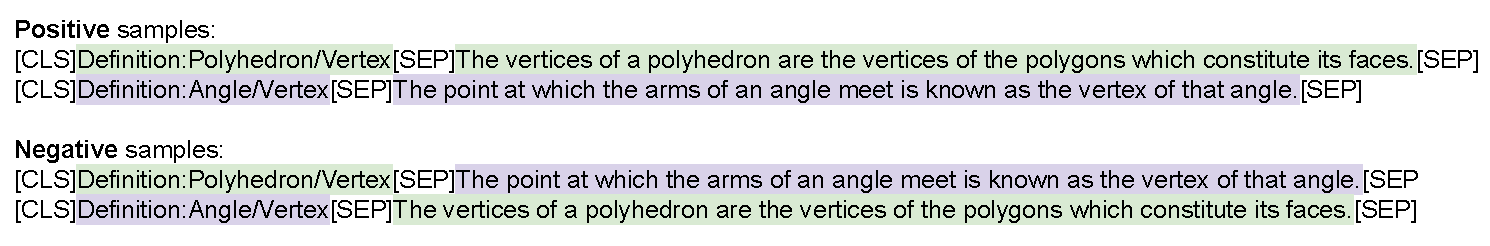
\includegraphics[width=\textwidth]{Fig/data_samples.pdf}
\caption{Sample training data made from the term ``Vertex''.} \label{fig:train_sample}
\end{figure}



results in two tables:
\begin{table}
    \centering
    \caption{Accuracy and macro F1 scores for prediction with (fine-tuned) BERT for NSP. Values are reported as $\rho \cdot 100$.}
    \begin{tabular}{|p{0.3\linewidth}|p{0.1\linewidth}|p{0.1\linewidth}|p{0.1\linewidth}|p{0.1\linewidth}|}
    \hline
        model name& \multicolumn{2}{l|}{Test} & \multicolumn{2}{l|}{Train}\\ \cline{2-5}
         & F1 & Acc. & F1 & Acc. \\ \hline
        BERT OOB & 80,9 & 84,8 & 79,8 & 83,9 \\ \hline
        BERT NSP 65ep & \textbf{92,1} & \textbf{93,8} & \textcolor{gray}{98,4} & \textcolor{gray}{98,7} \\ \hline
    \end{tabular}
    \label{tab:nsp_scores}
\end{table}

\begin{table}
    \centering
    \caption{Accuracy and macro F1 scores for prediction based on sentence embeddings produced with different models. Values are reported as $\rho \cdot 100$.}
    \begin{tabular}{|p{0.3\linewidth}|p{0.1\linewidth}|p{0.1\linewidth}|p{0.1\linewidth}|p{0.1\linewidth}|}
    \hline
        model name& \multicolumn{2}{l|}{Test} & \multicolumn{2}{l|}{Train}\\ \cline{2-5}
         & F1 & Acc. & F1 & Acc. \\ \hline
        BERT OOB & 26,1 & 35,3 & 30,2 & 40,3 \\ \hline
        CC-BERT ep10 & 28,2 & 37,9 & 35,6 & 45,4 \\ \hline
        all-MiniLM-L6-v2 & 90,1 & 92,4 & 88,1 & 91,0 \\ \hline
        all-MiniLM-L12-v2 & 91,2 & 93,3 & \textbf{89,4} & \textbf{92,1} \\ \hline
        all-mpnet-base-v2 & \textbf{91,4} & \textbf{93,5} & 89,0 & 91,6 \\ \hline
        Bert-MLM\_arXiv & 28,3 & 38,3 & 32,8 & 42,7 \\ \hline
        Bert-MLM\_arXiv-MP-class\_zbMath & 43,8 & 52,2 & 54,0 & 61,5 \\ \hline
    \end{tabular}
    \label{tab:sim_scores}
\end{table}

%%%%%%%%%%%%%%%%%%%%%%%%%%%%%%%%%%%%%%%%%%%%Eval begins
\sjdraft{discussion:}
Pre-training with MLM allows learning the representation of domain-specific text and improves downstream tasks when fine-tuning datasets are small~\cite{mishraPS21,jiang2022choubert}. However, most models pre-trained (from scratch with its tokenizer or further pre-trained with the initial weights of models in the general domain) with mathematical contents are built for and only evaluated with a specific downstream task. Thus, these models might not necessarily benefit other tasks.


\subsection{Limitation}
\label{sec:eval}
\begin{itemize}
    \item It is challenging to detect the semantic equivalence of mathematical statements. In our dataset, we only evaluate our approach on different definitions. 
    \item Though mathematical textbooks or other knowledge bases also contain definitions, since they are not aligned, we use only Proofwik disambiguation pages as ground truth dataset.
\end{itemize}


~\genet{SBERT-all-MiniLM-L6-v2 model is a lightweight and efficient model that achieves strong performance across tasks like semantic search, clustering, and text similarity\footnote{\url{https://huggingface.co/sentence-transformers/all-MiniLM-L6-v2}}. Pre-trained on a diverse dataset, it generalizes well to multiple domains without the need for extensive fine-tuning. Its counterpart, the SBERT-all-MiniLM-L12-v2 model, achieves even better accuracy due to its deeper architecture, with additional layers that capture more complex sentence representations. This added depth enhances its ability to grasp subtle nuances in meaning, making it especially effective for tasks like semantic similarity and sentence pair classification.}
%%%%%%%%%%%%%%%%%%%%%%%%%%%%%%%%%%%%%%%%%Eval ends